%!TEX program = pdflatex
\documentclass[11pt,en]{elegantpaper}

\title{The Report for Programming Assignments in Chapter One}
\author{Wenchong Huang}

\date{\today}

% cmd for this doc
\usepackage{array}
\usepackage{float}
\newcommand{\ccr}[1]{\makecell{{\color{#1}\rule{1cm}{1cm}}}}

\begin{document}

\maketitle


\section{How to Test}

Enter the folder \verb|Programming-Chapter1/src| with terminal, \verb |make| here, you will see some executable files whose names are corresponding assignments. Run them directly and you will see the results.

\section{Manual}

This package is for solving equations $f(x)=0$.

You should include the header \verb|EquationSolver.h|, then define your function object as a derived class of \verb|Function|. The deriviate function is an optional. If you didn't define the deriviate function but still use Newton's Method, the solver will use difference quotient to replace your derivate. Here is an example where $f(x)=x^{-1}-\tan x$.

\begin{lstlisting}
class F : public Function{
public:
    double operator () (const double &x) const{
        return 1.0/x-tan(x);
    }
    double diff (const double &x) const{
        return -1.0/(x*x) - 1.0/(cos(x)*cos(x));
    }
} f;
\end{lstlisting}

You could use Bisection Method to solve the equation $f(x)=0$, as following, where the \verb|a|, \verb|b|, \verb|delta| , \verb|eps| and \verb|M| are $a,b,\delta,\varepsilon$ and $M$ in the Algorithm 1.1 of the textbook.

\begin{lstlisting}
  BisectionSolver sol(f, a, b, delta, eps, M);
  double ans = sol.solve();
\end{lstlisting}

You may also try Newton's Method, as following, where the \verb|x0| , \verb|eps| and \verb|M| are $x_0,\varepsilon$ and $M$ in the Algorithm 1.14 of the textbook.

\begin{lstlisting}
  NewtonSolver sol(f, x0, eps, M);
  double ans = sol.solve();
\end{lstlisting}

You may also try Secant Method, as following (Don't ask why the name is \verb|SecandMethod|, that's a secre\textbf{d}.), where the \verb|x0|, \verb|x1|, \verb|delta| , \verb|eps| and \verb|M| are $x_0,x_1,\delta,\varepsilon$ and $M$ in the Algorithm 1.19 of the textbook.

\begin{lstlisting}
  SecandSolver sol(f, x0, x1, delta, eps, M);
  double ans = sol.solve();
\end{lstlisting}

Additional, if you don't want the solver's outputs to disturb you, you can add
\begin{lstlisting}
#define SILENCE
\end{lstlisting}
before including this package.

\section{Results}

\subsection{Assignment B}

The results see the following table, where the $\delta$ and $\varepsilon$ are all chose to be the machine precision.

\begin{table}[htbp]
  \centering
  \begin{tabular}{|c|c|c|c|c|c|}
  \hline
  \textbf{$f(x)$}                         & \textbf{$[a,b]$}    & \textbf{$x^*$} & \textbf{$f(x^*)$}       & \textbf{$k$} & \textbf{$|b_k-a_k|$}     \\ \hline
  $x^{-1}-\tan x$                         & $[0,\frac{\pi}{2}]$ & $0.860334$     & $0$                     & $53$         & $3.33067\times 10^{-16}$ \\ \hline
  $x^{-1}-2^x$                            & $[0,1]$             & $0.641186$     & $0$                     & $52$         & $4.44089\times 10^{-16}$ \\ \hline
  $2^{-x}+e^x+2\cos x-6$                  & $[1,3]$             & $1.82938$      & $0$                     & $53$         & $4.44089\times 10^{-16}$ \\ \hline
  $\frac{x^3+4x^2+3x+5}{2x^3-9x^2+18x-2}$ & $[0,4]$             & $0.116378$     & $6.08536\times 10^{15}$ & $56$         & $1.11022\times 10^{-16}$ \\ \hline
  \end{tabular}
\end{table}

The Bisection Method performs well at the first three functions, but fails at the last. That's because the precondition $\text{sgn}(f(a))\neq \text{sgn}(f(b))$ was not satisfied. Infact the last function has no root in interval $[0,4]$. See the following image.

\begin{figure}[htbp]
  \centering
  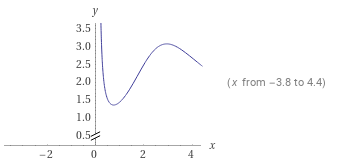
\includegraphics[width=0.4\textwidth]{image/fig1.png}
  \caption{The image of the last function.}
\end{figure}

\subsection{Assignment C}

The results see the following table.

\begin{table}[htbp]
  \centering
  \begin{tabular}{|c|c|c|c|c|}
  \hline
  \textbf{$f(x)$}             & \textbf{$x_0$} & \textbf{$x^*$} & \textbf{$f(x^*)$}         & \textbf{$k$} \\ \hline
  \multirow{2}{*}{$x-\tan x$} & $4.5$          & $4.49341$      & $-8.88178\times 10^{-16}$ & $4$          \\ \cline{2-5} 
                              & $7.7$          & $7.72525$      & $2.30926\times 10^{-14}$  & $5$          \\ \hline
  \end{tabular}
\end{table}

The Newton's Method converges fast as expected.

\subsection{Assignment D}

The results see the following table.

\begin{table}[htbp]
  \centering
  \begin{tabular}{|c|c|c|c|c|c|c|}
  \hline
  \textbf{$f(x)$}  & \textbf{$x_0$} & \textbf{$x_1$}  & \textbf{$x^*$} & \textbf{$f(x^*)$}         & \textbf{$k$} & \textbf{$|x_k-x_{k-1}|$} \\ \hline
  $sin(x/2)-1$     & $0$            & $\frac{\pi}{2}$ & $3.14159$      & $-1.11022\times 10^{-16}$ & $38$         & $1.50313\times 10^{-8}$  \\ \hline
  $e^x-\tan x$     & $1$            & $1.4$           & $1.30633$      & $-4.44089\times 10^{-16}$ & $17$         & $0$                      \\ \hline
  $x^3-12x^2+3x+1$ & $0$            & $-0.5$          & $-0.188685$    & $0$                       & $9$          & $0$                      \\ \hline
  \end{tabular}
\end{table}

We could try other initial values and get different results. See the following table.

\begin{table}[htbp]
  \centering
  \begin{tabular}{|c|c|c|c|c|c|c|}
  \hline
  \textbf{$f(x)$}                   & \textbf{$x_0$} & \textbf{$x_1$} & \textbf{$x^*$} & \textbf{$f(x^*)$}        & \textbf{$k$} & \textbf{$|x_k-x_{k-1}|$} \\ \hline
  $sin(x/2)-1$                      & $5.2\pi$       & $5.5\pi$       & $15.708$       & $0$                      & $37$         & $3.65908\times 10^{-8}$  \\ \hline
  $e^x-\tan x$                      & $-1.4$         & $-1.5$         & $-59.6903$     & $1.22588\times 10^{-15}$ & $15$         & $0$                      \\ \hline
  \multirow{2}{*}{$x^3-12x^2+3x+1$} & $0$            & $0.5$          & $0.451543$     & $2.22045\times 10^{-16}$ & $9$          & $1.11022\times 10^{-16}$ \\ \cline{2-7} 
                                    & $10$           & $11$           & $11.7371$      & $1.63425\times 10^{-13}$ & $10$         & $0$                      \\ \hline
  \end{tabular}
\end{table}

The results are easy to understand. The function $sin(x/2)-1$ vanishes at every point $(4k+1)\pi\;(k\in\mathbb{Z})$. The function $e^x-\tan x$ has a root at each interval $[k\pi-\frac{\pi}{2},k\pi+\frac{\pi}{2}]\;(k\in \mathbb{Z})$. And the polynimial function $x^3-12x^2+3x+1$ has three different real roots.

\subsection{Assignment E}

First define function $f(h)=L\left[0.5\pi r^2 - r^2 \text{arcsin} \frac{h}{r}-h(r^2-h^2)^{\frac{1}{2}}\right]-V$.

To make Newton's Method more efficient, we calculated the derivate by hand.

\begin{equation*}
  f'(h)= L\left[-\frac{r}{\sqrt{1-\left(\frac{h}{r}\right)^2}}-\sqrt{r^2-h^2}+\frac{2h^2}{\sqrt{r^2-h^2}}\right]
\end{equation*}

The results see the following table.

\begin{table}[H]
  \centering
  \begin{tabular}{|c|c|c|c|c|c|c|}
  \hline
  \textbf{}                 & \textbf{$[a,b]$} & \textbf{$x_0$} & \textbf{$x_1$} & \textbf{$x^*$} & \textbf{$f(x^*)$} & \textbf{$k$} \\ \hline
  \textbf{Bisection Method} & $[0,1]$          & *              & *              & $0.167969$     & $-0.0355476$      & $8$          \\ \hline
  \textbf{Newton's Method}  & *                & $0$            & *              & $0.166177$     & $-0.000215002$    & $2$          \\ \hline
  \textbf{Secant Method}    & *                & $0$            & $0.5$          & $0.16623$      & $-0.00126434$     & $3$          \\ \hline
  \end{tabular}
\end{table}

\subsection{Assignment F}

The function $f(x)$ defines as following.

\begin{equation*}
  f(x)=A\sin x\cos x+B \sin^2 x - C\cos x - E\sin x
\end{equation*}

Also, to make Newton's Method more efficient, we calculated the deriviate by hand.

\begin{equation*}
  f'(x)=A(-\sin^2 x + \cos^2 x) + 2B\cos x\sin x + C\sin x - E\cos x
\end{equation*}

The results see the following table.

\begin{table}[htbp]
  \centering
  \begin{tabular}{|cc|c|c|c|c|c|}
  \hline
  \multicolumn{2}{|c|}{\textbf{}}                      & \textbf{$x_0$} & \textbf{$x_1$} & \textbf{$x^*$}              & \textbf{$f(x^*)$} & \textbf{$k$} \\ \hline
  \multicolumn{1}{|c|}{\textbf{(a)}} & Newton's Method & $33^\circ$     & *              & $0.575473\;(32.9722^\circ)$ & $0$               & $3$          \\ \hline
  \multicolumn{1}{|c|}{\textbf{(b)}} & Newton's Method & $33^\circ$     & *              & $0.578907\;(33.1689^\circ)$ & $0$               & $5$          \\ \hline
  \multicolumn{1}{|c|}{\textbf{(c)}} & Secant Method   & $30^\circ$     & $33^\circ$     & $0.575473\;(32.9722^\circ)$ & $0$               & $5$          \\ \hline
  \end{tabular}
\end{table}

We tried another initial value at problem (c), the result sees following.

\begin{table}[htbp]
  \centering
  \begin{tabular}{|cc|c|c|c|c|c|}
  \hline
  \multicolumn{2}{|c|}{\textbf{}}                                                      & \textbf{$x_0$} & \textbf{$x_1$} & \textbf{$x^*$}             & \textbf{$f(x^*)$}         & \textbf{$k$} \\ \hline
  \multicolumn{1}{|c|}{\multirow{3}{*}{\textbf{(c)}}} & \multirow{3}{*}{Secant Method} & $0^\circ$      & $5^\circ$      & $-0.200713\;(-11.5^\circ)$ & $0$                       & $9$          \\ \cline{3-7} 
  \multicolumn{1}{|c|}{}                              &                                & $100^\circ$    & $120^\circ$    & $2.56612\;(147.028^\circ)$ & $-3.55271\times 10^{-15}$ & $9$          \\ \cline{3-7} 
  \multicolumn{1}{|c|}{}                              &                                & $180^\circ$    & $170^\circ$    & $2.94088\;(168.5^\circ)$   & $-1.77636\times 10^{-15}$ & $8$          \\ \hline
  \end{tabular}
  \end{table}

Actually, the function is periodic function with period $2\pi$, and it has four different roots at each period. The image sees following.

\begin{figure}[htbp]
  \centering
  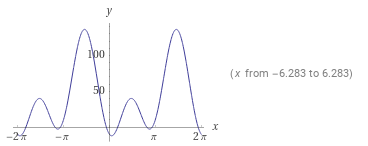
\includegraphics[width=0.4\textwidth]{image/fig2.png}
  \caption{The image of the function in problem (c).}
\end{figure}

\section{Summary}

This template is designed by Elegant\LaTeX{} Program.

Many appreciations for your carefully reading. If you found any mistakes, please contact me directly. Have fun with your loving one (boyfriend, girlfriend or coding)!

\end{document}
